\newpage
% 1. Разработать технологию тестирования системы
% 2. Разработать технологии развертывания и использования системы

\section{Разработка технологий тестирования}
\label{sec:technolog}

\subsection{Технология тестирования работы системы}

Согласно техническому заданию требуется разработать технологию тестирования работы системы.
Также в соответствии с ТЗ необходимо выполнить тестирование корректности взаимодействия (интеграции) программной и аппаратной частей, которое направлено на проверку корректности работы обмена данными между мобильным приложением, считывателем бесконтактных карт и сервером банка-эквайера.

Технология тестирования разработанной программно-аппаратной системы представляет последовательную проверку корректности работы основных функциональных модулей посредством воспроизведения тестирующих сценариев с их использованием.
Основные модули разработанной системы:

\begin{itemize}
	\item модуль взаимодействия по Bluetooth мобильного приложения, используемого для подключения мобильного устройства к считывателю;
	\item модуль платежных операций мобильного приложения, используемого для интеграции с сервером банка посредством REST API;
	\item модуль управления мобильным приложением, используемого для управления логикой отображения интерфейса и взаимодействия с ним;
	\item модуль взаимодействие с приложением на мобильном устройстве посредством Bluetooth считывателя бесконтактных средств платежа;
	\item модуль взаимодействия с бесконтактным средством платежа посредством NFC считывателя бесконтактных средств платежа;
	\item модуль установления соединения с бесконтактной картой по стандарту ISO/IEC 14443 считывателя бесконтактных средств платежа;
	\item модуль взаимодействия с картой ПС <<МИР>> для выполнения платежной операции считывателя бесконтактных средств платежа.
\end{itemize}


Для реализации данной технологии тестирования необходимо выполнить следующие этапы:

\begin{enumerate}
	\item настройка среды эмуляции ответов сервера банка~--- создание сервера-заглушки для имитации поведение REST API сервера банка, чтобы протестировать возможные сценарии выполнения платежной транзакции: запрос проверки PIN-кода, запрос проверки подписи, успешное выполнение платежной транзакции, различные ошибки выполнения платежной транзакции;
	\item проверка работы логирования в Android--приложении (вывод в Logcat) и на устройстве-считывателе (вывод на UART интерфейс, подключенный к эмулируемому ПК COM-портом);

	\item подготовка макета устройства~--- запуск тестирования работы программных процедур аппаратной части системы, тестовые случаи для которых описаны в подразделе~\ref{subsec:des_test}, посредством запуска тестирующей версии программного обеспечения МК;
	\item установка прошивки на макет устройства~--- загрузка исполняемой программы на микроконтроллер и проверка его запуска;

	\item подготовка к запуску мобильного приложения~--- запуск структурного и модульного тестирования процедур мобильного приложения с помощью средств Android Studio и библиотеки JUnit, тестовые случаи для которых описаны в подразделе~\ref{subsec:des_test};
	\item установка и запуск программы на мобильном устройстве или его эмуляторе~--- установка исполняемого apk-файла приложения на устройство или эмулятор;

	\item выполнение тестовых сценариев.
\end{enumerate}

Сервер-заглушка для имитации поведение REST API сервера банка создается с помощью приложения Mockoon, предназначенного для ПК.
Оно позволяющего запускать сервер в локальной сети, к которому можно подключаться с других устройств, находящихся в этой же сети.
Интерфейс приложения с примером ответа на запрос представлен на рисунке~\ref{fig:mockoon}.

\begin{figure}[h]
	\centering
	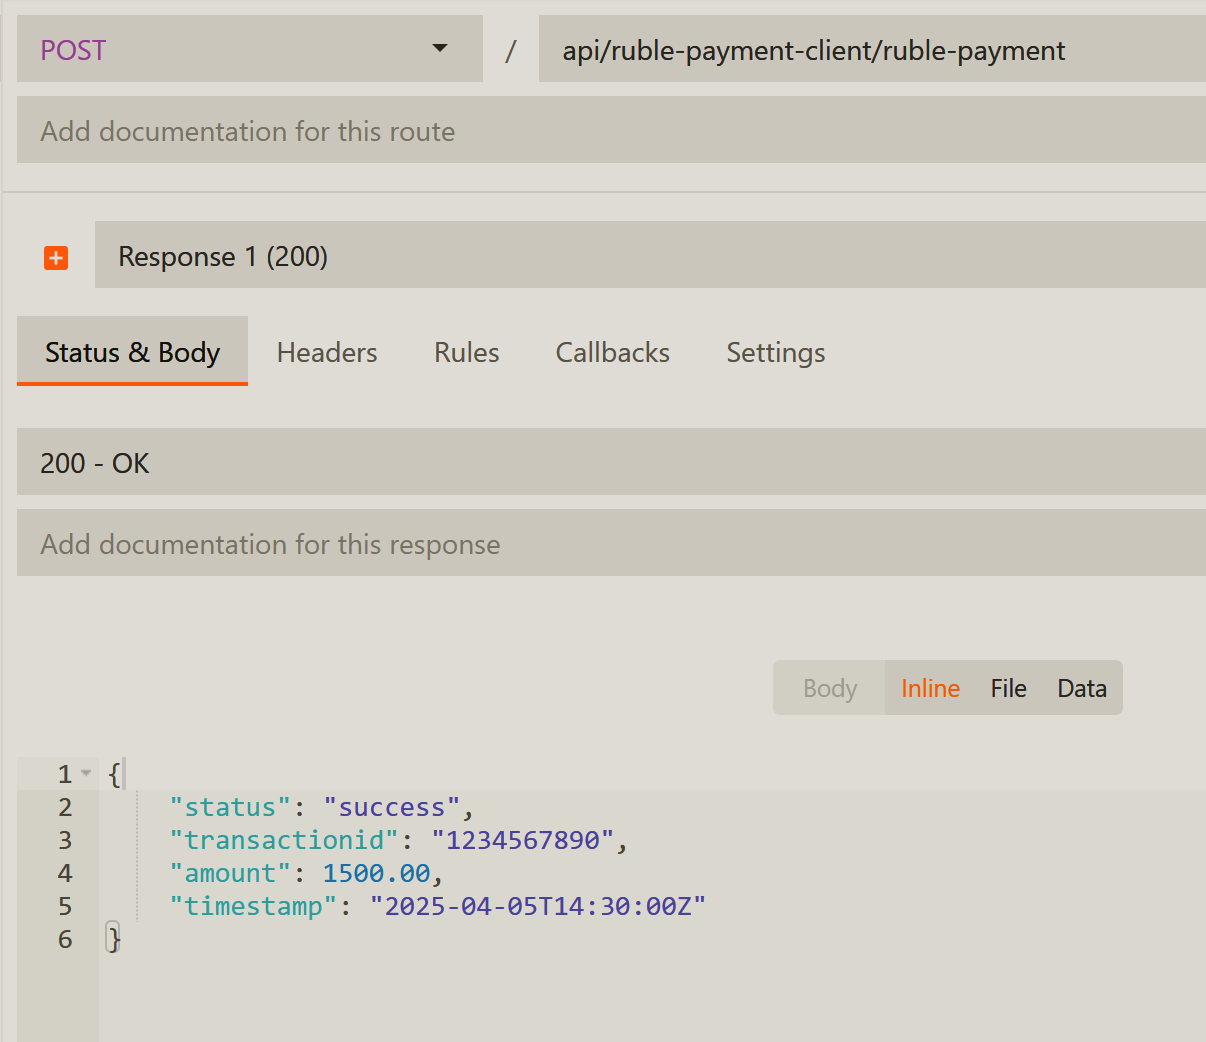
\includegraphics[width=0.7\textwidth]{images/technological/mockoon}
	\caption{\centering HTTPS маршрут-заглушка в приложении Mockoon}
	\label{fig:mockoon}
\end{figure}


Был разработан набор автономных тестовых сценариев, использующих ответы сервера-заглушки, чтобы проверить все варианты развития транзакции без прямого доступа к реальному банку.

Тестовый сценарий 1: подключение к считывателю по Bluetooth.
Ожидаемая реакция: успешное подключение к считывателю, отображение статуса <<Подключено>>.
Полученный результат: подключение установлено, состояние устройства обновлено, можно продолжить создание платежа.
Алгоритм тестирования:
\begin{enumerate}
	\item в мобильном приложении пользователь переходит на экран выбора устройства;
	\item активируется поиск доступных Bluetooth-устройств;
	\item пользователь выбирает устройство-считыватель из списка найденных.
\end{enumerate}

Тестовый сценарий 2: инициализация бесконтактной карты через NFC.
Ожидаемая реакция: карта успешно обнаружена, выполняется антиколлизия (ISO/IEC 14443--3), инициализация (ISO/IEC 14443--4) и получение UID карты.
Полученный результат: уникальный идентификатор карты получен, карта активирована, в приложении выполнен переход на экран успешного обнаружения карты.
Алгоритм тестирования:
\begin{enumerate}
	\item пользователь запускает платежную операцию в мобильном приложении;
	\item считыватель активирует NFC-модуль;
	\item пользователь подносит бесконтактную карту <<МИР>> к считывателю.
\end{enumerate}

Тестовый сценарий 3: чтение данных с карты и формирование запроса к серверу банка.
Ожидаемая реакция: корректная передача данных с карты, формирование защищённого HTTPS-запроса к серверу.
Полученный результат: данные успешно получены, формат запроса — JSON, отправка выполнена через HTTPS-соединение.
Алгоритм тестирования:
\begin{enumerate}
	\item после успешного обмена командами SELECT AID, GET PROCESSING OPTIONS, READ RECORD считыватель отправляет команду GENERATE AC для получения данных для формирования платежа;
	\item считыватель получает ответ на команду и передает его на мобильное устройство;
	\item мобильное приложение получает данные: Application Cryptogram, сумму, срок действия, условия использования и формирует JSON-запрос к серверу банка-эквайера через REST API.
\end{enumerate}

Тестовый сценарий 4: платёж с вводом PIN-кода и его онлайн верификацией.
Ожидаемая реакция: PIN шифруется и отправляется на сервер эквайера для верификации.
Полученный результат: PIN передан в зашифрованном виде, банк вернул положительный ответ.
Алгоритм тестирования:
\begin{enumerate}
	\item в ходе успешного выполнения Transaction Flow установлено, что сумма платежа превышает лимит офлайн-оплаты;
	\item карта запрашивает онлайн-PIN через CVM Results;
	\item считыватель получает запрос от карты и передает в мобильное приложение;
	\item мобильное приложение открывает экран ввода PIN-кода;
	\item пользователь вводит правильный PIN.
\end{enumerate}

Тестовый сценарий 5: офлайн-оплата без ввода PIN.
Ожидаемая реакция: транзакция завершается локально, без обращения к серверу.
Полученный результат: транзакция одобрена, выводится экран успеха.
Алгоритм тестирования:
\begin{enumerate}
	\item пользователь создаёт платёж на сумму ниже лимита, позволяющего провести операцию без PIN;
	\item карта проходит Dynamic Data Authentication (DDA);
	\item считыватель формирует TC (Transaction Certificate).
\end{enumerate}

Тестовый сценарий 6: отказ в проведении транзакции.
Ожидаемая реакция: мобильное приложение отображает экран ошибки с причиной отклонения транзакции.
Полученный результат: транзакция отклонена, в мобильном приложении отображает экран ошибки с причиной отклонения транзакции.
Алгоритм тестирования:
\begin{enumerate}
	\item пользователь пытается оплатить просроченной картой;
	\item считыватель получает флаг Application Expired или не проходит Processing Restrictions
	\item считыватель отправляет отправляет информацию об этом в мобильное приложение.
\end{enumerate}

Тестовый сценарий 7: неудачное подключение к считывателю.
Ожидаемая реакция: приложение отображает сообщение <<Не удалось подключиться к считывателю>>.
Полученный результат: сообщение отображается, пользователь может повторить попытку или выбрать другое устройство.
Алгоритм тестирования:
\begin{enumerate}
	\item пользователь пытается подключиться к считывателю, к которому подключено другое устройство;
	\item мобильное приложение выполняет попытку подключения;
	\item происходит таймаут подключения.
\end{enumerate}

Тестовый сценарий 8: обрыв Bluetooth-соединения во время транзакции.
Ожидаемая реакция: система информирует пользователя о потере связи, транзакция отменяется.
Полученный результат: связь потеряна, транзакция отменена, приложение готово к повторному запуску.
Алгоритм тестирования:
\begin{enumerate}
	\item пользователь начинает процесс оплаты;
	\item Bluetooth-соединение обрывается во время обнаружения карты;
	\item мобильное приложение детектирует разрыв.
\end{enumerate}

Тестовый сценарий 9: запрос подписи держателя карты.
Ожидаемая реакция: подпись отправлена, банк проверяет подлинность и возвращает статус.
Полученный результат: подпись успешно передана, сервер вернул статус <<Успешно>>.
Алгоритм тестирования:
\begin{enumerate}
	\item сумма платежа превышает лимит, при котором требуется дополнительная верификация;
	\item карта запрашивает ввод подписи (CVM Type = ‘1E’);
	\item мобильное приложение открывает экран ввода подписи;
	\item подпись отправляется в запросе на сервер банка-эквайера.
\end{enumerate}

Тестовый сценарий 10: Получение UID карты по стандарту ISO/IEC 14443--3 с последующей активацией карты по стандарту ISO/IEC 14443--4.
Ожидаемая реакция: карта успешно идентифицирована, UID записан в контекст транзакции.
Полученный результат: уникальный идентификатор карты успешно прочитан, выполнен переход к экрану успешного обнаружения карты.
Алгоритм тестирования:
\begin{enumerate}
	\item пользователь подносит карту к считывателю;
	\item считыватель выполняет обнаружение карты и антиколлизию;
	\item считыватель получает UID;
	\item считыватель инициирует протокол ISO/IEC 14443--4 для установления логического канала связи (отправляет команду RATS);
	\item считыватель получает ответ карты ATS;
	\item считыватель передает ответ карты в мобильное приложение.
\end{enumerate}


\subsection{Интеграционное тестирование}
\label{subsec:test_integr}

Проверка интеграции считывателя с мобильным приложением происходит посредством проверки наличия подключения и его корректной работы между мобильным устройством и считывателем посредством отправки тестовых сообщений с выводом в логи мобильного приложения и считывателя и их последующего сравнения.
Для логирования Android--приложения используется инструмент Logcat, предоставляемой Android Studio, используемой для разработки приложения, для логирования работы считывателя используется вывод на UART интерфейс, подключенный к эмулируемому ПК COM-портом.

Сохранение логов мобильного приложения происходит в отдельный файл посредством использования скрипта, представленного в листинге~\ref{code:test_andr}.

\begin{singlespacing}
	\small
	\captionsetup{labelsep=endash, justification=raggedright, singlelinecheck=off}
	\lstinputlisting[language=c++, label=code:test_andr, linerange={1-39}, caption={Сохранения логов мобильного приложения}]{code/test_andr.cpp}
\end{singlespacing}

Логирование МК осуществляется путем настройки UART на STM32, используя STM32CubeIDE.
Реализация передачи данных выполняется посредством функции HAL\_UART\_Transmit.
Отладочная плата Blue Pill, используемая в макете, подключается через USB-TTL преобразователь к UART входу.
Определяется COM-порт, к которому происходит подключение.
С помощью скрипта, представленного в листинге~\ref{code:test_pos}, происходит сохранение логов в файл (также это возможно в некоторых терминалах, таких как Tera Term, PuTTY, посредством опции Log to File).

\begin{singlespacing}
	\small
	\captionsetup{labelsep=endash, justification=raggedright, singlelinecheck=off}
	\lstinputlisting[language=python, label=code:test_pos, linerange={1-15}, caption={Сохранения логов считывателя}]{code/test_pos.py}
\end{singlespacing}


Выполнение данной процедуры производилось при различной удаленности и, как следствие, силе сигнала Bluetooth.
В результате тестирования не выявлено критических ошибок, связанных с потерей данных или нарушением целостности транзакции.
Все этапы обмена данными между программной и аппаратной частью выполняются корректно и соответствуют требованиям безопасности, установленными в ТЗ.
